\chapter{Годограф Найквиста}
\label{ch:chap1}
\newcommand\tab[1][1cm]{\hspace*{#1}}

\ExplSyntaxOn
\clist_new:N \l_feq_vector_clist
\NewDocumentCommand{\feqvector}{O{\\}mO{b}}{
  \clist_set:Nn \l_feq_vector_clist {#2} % Set the list
  \begin{#3matrix}
  \clist_use:Nn \l_feq_vector_clist {#1} % show it with separator from #1 (\\)
  \end{#3matrix}
}
\ExplSyntaxOff

Параметры для объектов:
$$
  p=1, \tab q=4, \tab n=4, \tab m=1
$$

Нам нужно придумать три объекта пятого порядка, который будет иметь $p$ вещественных полюсов передаточных функций и $q$ - комплексно-сопряжённых. 
Но у каждого из объектов будет своё соотношение неустойчивых полюсов у замкнутой и разомкнутой системы.

\section{Система первая}

\subsection{Передаточная функция}

Выпишем передаточную функцию для разомкнутой системы 5-го порядка в общем виде:
$$
W_{open}(s) = \frac{s^5 + b_4s^4 + b_3s^3 + b_2s^2 + b_1s + b_0}{s^5 + a_4s^4 + a_3s^3 + a_2s^2 + a_1s + a_0}
$$
В замкнутом виде она несколько изменится:
$$
\begin{aligned}
  W_{closed}(s) = \frac{1}{1+W} =\\ 
  \frac{s^5 + a_4s^4 + a_3s^3 + a_2s^2 + a_1s + a_0}{2s^5 + (a_4 + b_4)s^4 + (a_3 + b_3)s^3 + (a_2 + b_2)s^2 + (a_1 + b_1)s + (a_0 + b_0)}
\end{aligned}
$$

В нашем случае мы пока можем записать только передаточную функцию с интересующими нас полюсами:
$$
W_{open}(s) = \frac{(s-\lambda_1)(s-\lambda_2)(s-\lambda_3)(s-\lambda_4)(s-\lambda_5)}{(s-\gamma)(s-z_1)(s-\overline{z}_1)(s-z_2)(s-\overline{z}_2)}
$$
% Для простоты возьмём все нули - с левыми корнями, то $\lambda_i < 0$.

Пару комплексных корней мы перепишем несколько иначе, раскрыв их как $z_i = a_i + jb_i$ :
$$
W_{open}(s) = \frac{(s-\lambda_1)(s-\lambda_2)(s-\lambda_3)(s-\lambda_4)(s-\lambda_5)}{(s-\gamma)( (s-\alpha_1)^2 +\beta_1^2)( (s-\alpha_2)^2 +\beta_2^2)}
$$
По условию моего варианта система в разомкнутом виде должна иметь 1 вещественный и 4 комплексно-сопряжённых полюса. В разомкнутом виде у нас должно быть 4 неустойчивых полюса. 

А значит,  $\gamma < 0$, $\alpha_{1,2} > 0$, чтобы выполнить это условие.

Тогда естественным образом выразится ПФ для замкнунтой системы:
$$
\begin{aligned}
  W_{closed}(s) = \\
  \frac{(s-\lambda_1)(s-\lambda_2)(s-\lambda_3)(s-\lambda_4)(s-\lambda_5)}{ (s-\lambda_1)(s-\lambda_2)(s-\lambda_3)(s-\lambda_4)(s-\lambda_5) + (s-\gamma)( (s-\alpha_1)^2 +\beta_1^2)( (s-\alpha_2)^2 +\beta_2^2) }
\end{aligned}
$$
В разомкнутом виде у нас должен быть 1 неустойчивый полюс. Здесь уже явно не наложишь ограничения на параметры, поэтому придётся раскрывать скобки и расписывать\dots

Надо придумать такой способ перевода между коэффициентами полинома 5-й степени и его корнями, для этого просто распишем полином в общем виде:
\small
$$
\begin{aligned}
  (s-\lambda_1)(s-\lambda_2)(s-\lambda_3)(s-\lambda_4)(s-\lambda_5) = \\
  s^5 
  \\+ (-\lambda_1-\lambda_2-\lambda_3-\lambda_4-\lambda_5)s^4  
  \\+ (\lambda_1\lambda_4 + \lambda_1\lambda_3 + \lambda_2\lambda_3 + \lambda_2\lambda_4 + \lambda_1\lambda_2 + \lambda_3\lambda_5 + \lambda_4\lambda_5 + \lambda_1\lambda_5+ \lambda_2\lambda_5 + \lambda_3\lambda_4)s^3 
  \\+ (\lambda_1\lambda_3\lambda_4 + \lambda_2\lambda_3\lambda_4 + \lambda_1\lambda_2\lambda_3 + \lambda_1\lambda_2\lambda_4+ \lambda_3\lambda_4\lambda_5 \\
    + \lambda_1\lambda_4\lambda_5 + \lambda_1\lambda_3\lambda_5 + \lambda_2\lambda_3\lambda_5 + \lambda_2\lambda_4\lambda_5 + \lambda_1\lambda_2\lambda_5)s^2 
  \\+ (\lambda_1\lambda_2\lambda_3\lambda_4 + \lambda_1\lambda_2\lambda_4\lambda_5 + \lambda_1\lambda_2\lambda_3\lambda_5 + \lambda_2\lambda_3\lambda_4\lambda_5)s 
  \\+ \lambda_1\lambda_2\lambda_3\lambda_4\lambda_5
\end{aligned}
$$
\normalsize
Конечно, проще это будет воспринимать как вектор коэффициентов, иными словами:
\small
$$ 
\begin{pmatrix}
  -(\lambda_1+\lambda_2+\lambda_3+\lambda_4+\lambda_5) \\
  \lambda_1\lambda_4 + \lambda_1\lambda_3 + \lambda_2\lambda_3 + \lambda_2\lambda_4 + \lambda_1\lambda_2 + \lambda_3\lambda_5 + \lambda_4\lambda_5 + \lambda_1\lambda_5+ \lambda_2\lambda_5 + \lambda_3\lambda_4 \\ 
  \\+ \lambda_1\lambda_3\lambda_4 + \lambda_2\lambda_3\lambda_4 + \lambda_1\lambda_2\lambda_3 + \lambda_1\lambda_2\lambda_4+ \lambda_3\lambda_4\lambda_5 + \lambda_1\lambda_4\lambda_5 + \lambda_1\lambda_3\lambda_5 + \lambda_2\lambda_3\lambda_5 + \lambda_2\lambda_4\lambda_5 + \lambda_1\lambda_2\lambda_5  \\
  \lambda_1\lambda_2\lambda_3\lambda_4 + \lambda_1\lambda_2\lambda_4\lambda_5 + \lambda_1\lambda_2\lambda_3\lambda_5 + \lambda_2\lambda_3\lambda_4\lambda_5 \\
  \lambda_1\lambda_2\lambda_3\lambda_4\lambda_5 \\
\end{pmatrix}
$$
\normalsize

Также в знаменателе есть и второе слагаемое, которое также можно расписать в общем виде и разбить на вектор, состоящий из параметров $(\gamma, \alpha_1, \beta_1, \alpha_2, \beta_2)$, но делать мы этого не будем, а проще выберем конкретные значения, чтобы много не нагромождать формул:
\small
$$
(s-\lambda_1)(s-\lambda_2)(s-\lambda_3)(s-\lambda_4)(s-\lambda_5) + (s-\gamma)( (s-\alpha_1)^2 +\beta_1^2)( (s-\alpha_2)^2 +\beta_2^2)
$$
$$
(s-\lambda_1)(s-\lambda_2)(s-\lambda_3)(s-\lambda_4)(s-\lambda_5) + (s+5)( (s-3)^2 + 4 )( (s-4)^2 + 9)
$$
$$
(s-\lambda_1)(s-\lambda_2)(s-\lambda_3)(s-\lambda_4)(s-\lambda_5) + s^5 -9s^4 + 16s^3 +176s^2 -945s + 1625
$$
\normalsize
Дело за малым - суммируем два вектора коэффиентов: $\overline{\lambda} + \overline{\delta}$, запишем 
то в кратком виде, чтобы не переусердствовать с формулами:
$$
  2s^5 -9\overline{\lambda}_1s^4 + 16\overline{\lambda}_2s^3 +176\overline{\lambda}_3s^2 -945\overline{\lambda}_4s + 1625\overline{\lambda}_5
$$
Теперь надо подобрать такие $\lambda_i$, чтобы у числителя был 1 неустойчивый полюс. 
Чтобы облегчить поиск такой системы, я приравнял $\lambda_1=\lambda_2=\lambda_3=-1$, и настраивал уже только $\lambda_{4,5}$. 
С помощью \textit{matlab} получил, при:
$$
 \lambda_4= -1, \tab \lambda_5= 10
$$
Следующее уравнение в числителе:
$$
  2s^5 -\frac{42}{5}s^4-\frac{1521}{50}s^3-\frac{2993}{50}s^2-\frac{1041}{25}s-\frac{9}{5}
$$
Будет иметь следующие корни:
$$
  x_1 = -1, \tab x_2 \approx -0.05 ,\tab x_{3,4} \approx -0.9 \pm 1.4j, \tab x_5 \approx 7
$$
Всё сходится, тогда финально получим следующие две ПФ, подставив все значения:
$$
W_{open}(s) = \frac{s^5 -6s^4 -34s^3 -56s^2 -39s-10}{s^5 -\frac{12}{5}s^4+\frac{179}{50}s^3-\frac{193}{50}s^2-\frac{66}{25}s+\frac{41}{5}}
$$
$$
W_{closed}(s) = \frac{s^5 -6s^4 -34s^3 -56s^2 -39s-10}{2s^5 -\frac{42}{5}s^4-\frac{1521}{50}s^3-\frac{2993}{50}s^2-\frac{1041}{25}s-\frac{9}{5}}
$$
Для следующих систем мы сразу будем начинать с готовых ПФ, потому что алгоритм их производства будет аналогичным, за исключением выбора начальных корней.

\subsection{Карты полюсов}
\begin{figure}[h]
  \begin{subfigure}{0.5\textwidth}
    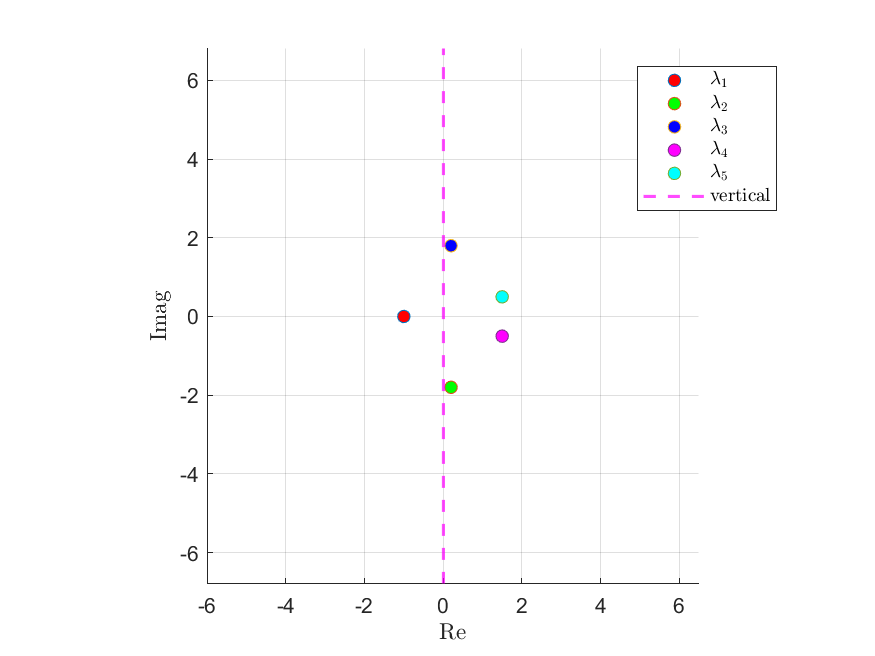
\includegraphics[width=0.9\linewidth]{roots_open1.png} 
    \caption{Разомкнутая система}
  \end{subfigure}
  \begin{subfigure}{0.5\textwidth}
    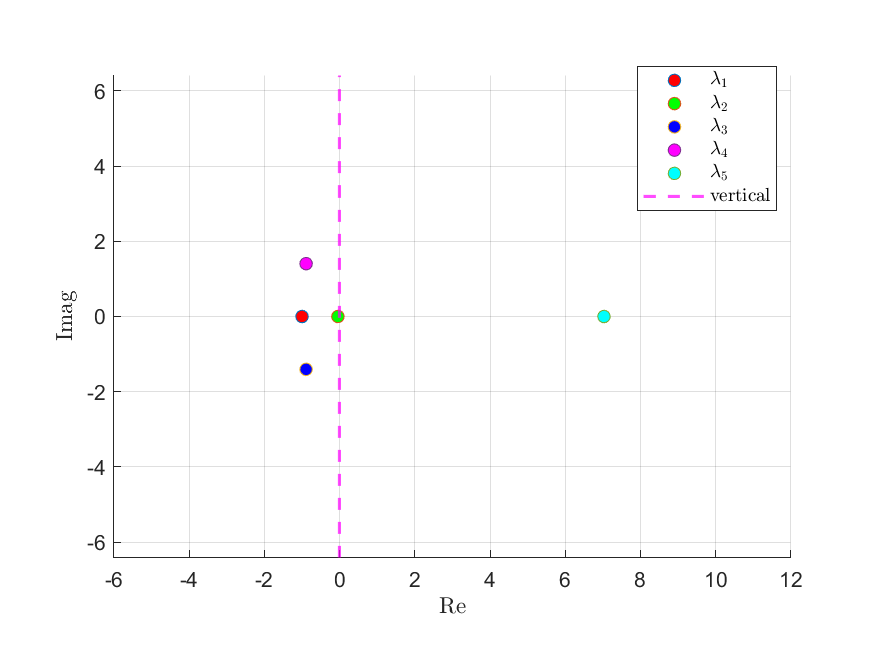
\includegraphics[width=0.9\linewidth]{roots_closed1.png}
    \caption{Замкнутая система}
  \end{subfigure}
  \caption{Карты полюсов для системы}
\end{figure}

\newpage
\subsection{Годограф Найквиста}
\begin{figure}[ht]
    \centering
    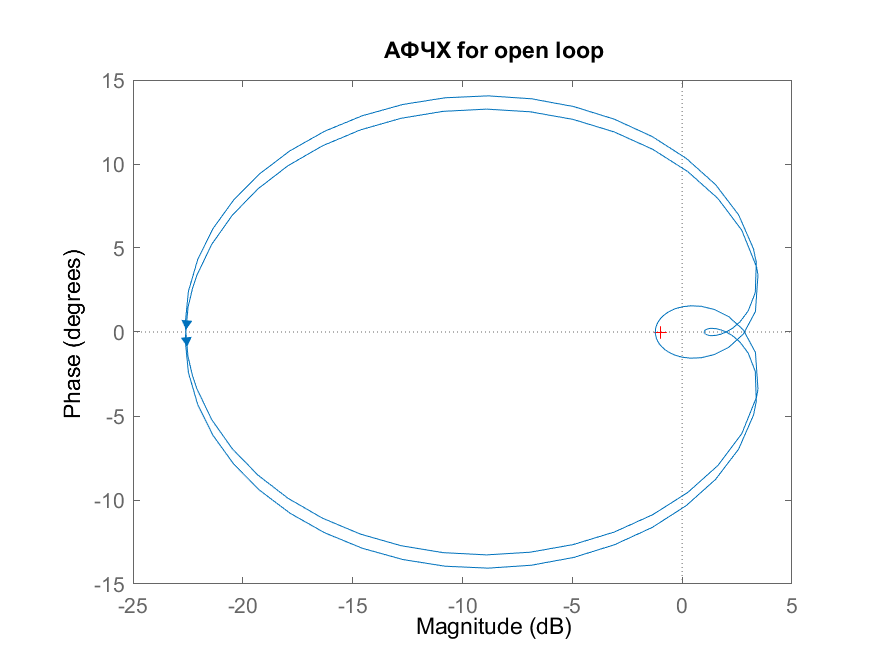
\includegraphics[width=1.0\textwidth]{nyquistplot_open1.png}
    \caption{Годограф Найквиста для системы}
  \end{figure}

Годограф Найквиста охватывает внутрь себя точку (-1, 0) и делает вокруг неё три оборота против часовой стрелки. 
По критерию Найквиста это значит, что у замкнутой системы количество неустойчивых полюсов станет на три меньше, чем у разомкнутой(было 4, станет 4-3=1 неустойчивых полюсов). 
Именно такой результат мы в итоге и получили.

\subsection{Переходные характеристики}

\begin{figure}[hbt!]
  \begin{subfigure}{.500\linewidth}
    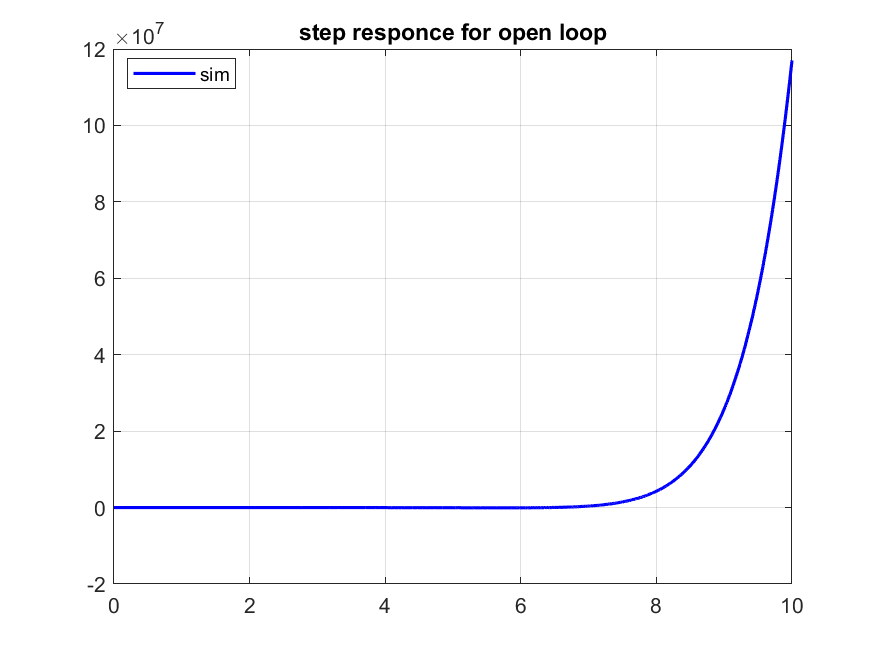
\includegraphics[width=\linewidth]{step_responce_open1.png}
    \caption{}
  \end{subfigure}\hfill % <-- "\hfill"
  \begin{subfigure}{.500\linewidth}
    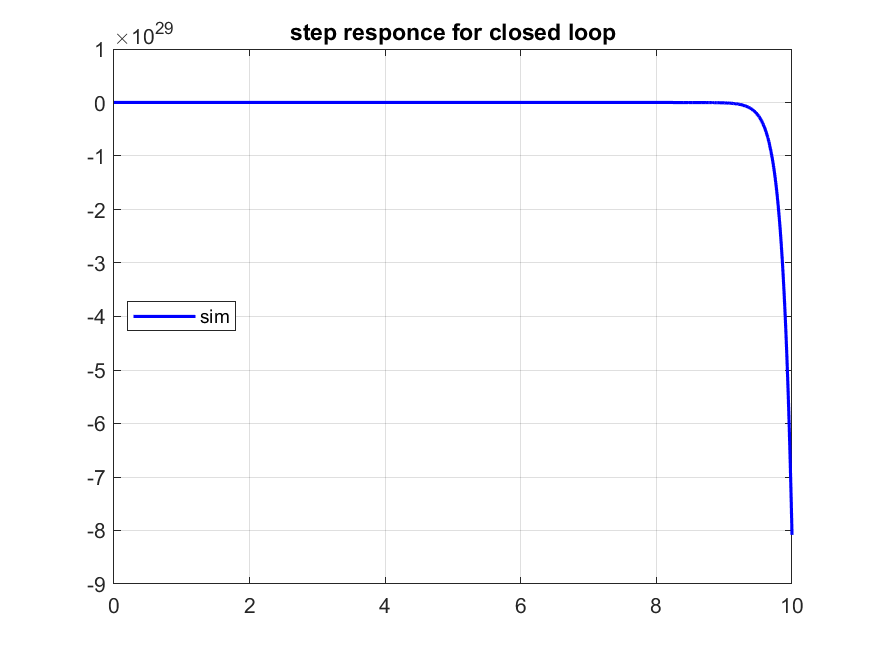
\includegraphics[width=\linewidth]{step_responce_closed1.png}
    \caption{}
  \end{subfigure}
  
  \medskip 
  \begin{subfigure}{.500\linewidth}
    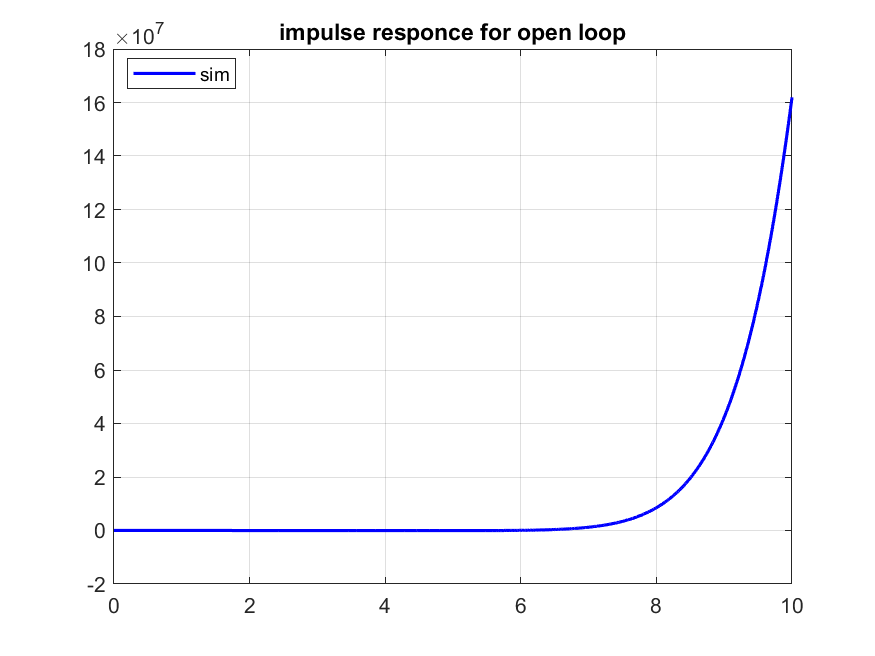
\includegraphics[width=\linewidth]{impulse_responce_open1.png}
    \caption{}
  \end{subfigure}\hfill 
  \begin{subfigure}{.500\linewidth}
    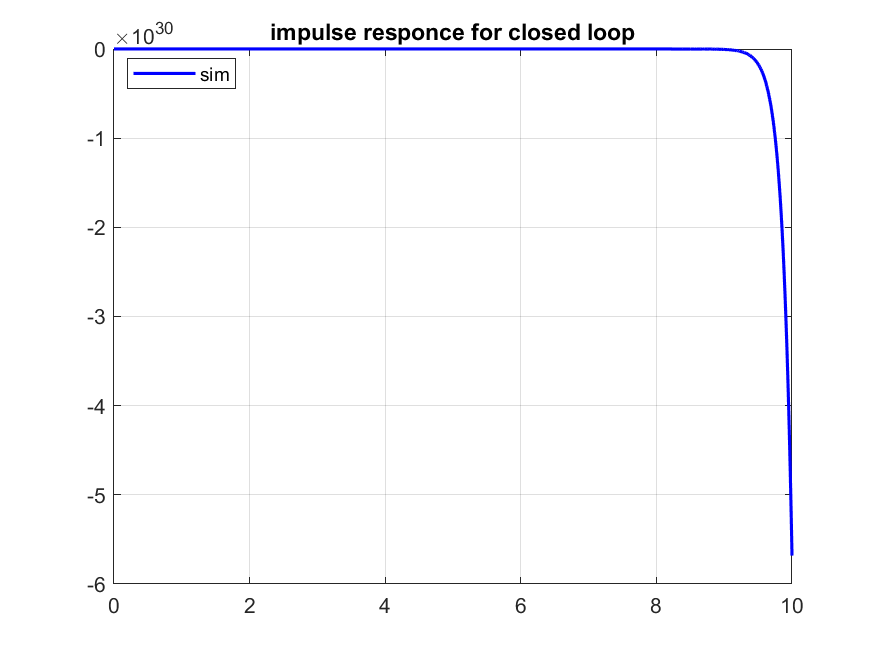
\includegraphics[width=\linewidth]{impulse_responce_closed1.png}
    \caption{}
  \end{subfigure}
  
  \caption{Сравнение - переходные характеристики}
  \label{fig:roc}
  \end{figure}
По переходным функциям можем сделать вывод, что системы, как разомкнутая, так и замкнутая неустойчивые.

\newpage
\subsection{Логарифмический критерий Найквиста}
Построим ЛАФЧХ для аналитики:
\begin{figure}[ht]
    \centering
    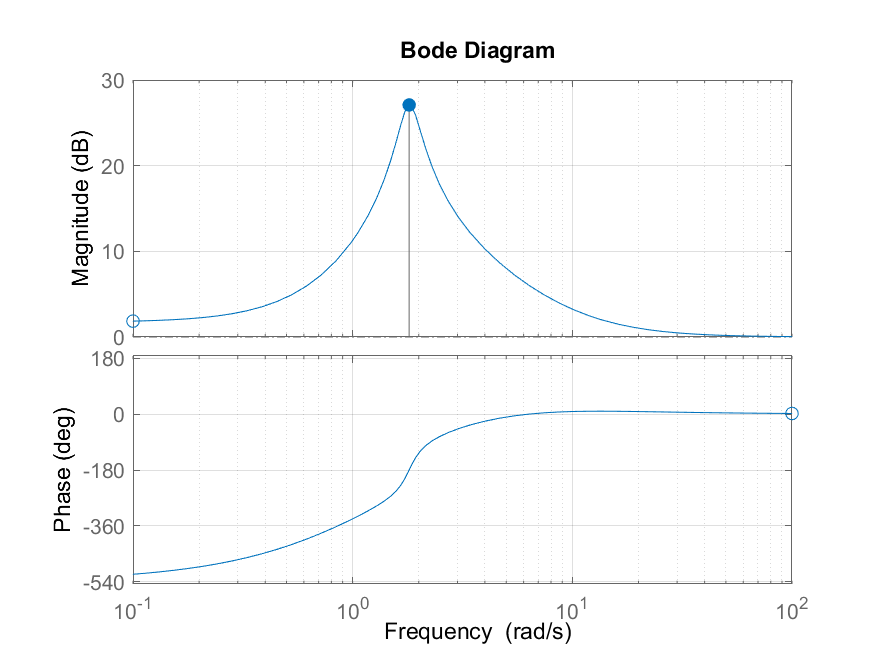
\includegraphics[width=1.0\textwidth]{log_nyquist1.png}
    \caption{ЛАФЧХ для системы}
  \end{figure}

Из графика делаем вывод, что система является неустойчивой по логарифмическому критерию Найквиста, 
мы стартуем из значения $-540^\circ$, что является критическим отрезком, значит мы считаем переход за $+\frac{1}{2}$, 
далее на отметке ЛФЧХ в $-180^\circ $ у нас будет положительных переход $+1$, но для устойчивости нам нужно, чтобы разность между переходами была равна $\frac{r}{2} = \frac{4}{2} = 2$, у нас будет $1.5 - 0 = 1.5$, этого недостаточно.
Уточню, что $r$ - количество правых корней для разомкнутой системы.
\newpage

\section{Система вторая}
Данная система должна иметь 0 неустойчивых полюсов у разомкнутой системы и 1 у замкнутой. 
Значит годограф Найквиста должен сделать один оборот по часовой стрелке вокруг $(-1, 0)$.
\subsection{Передаточная функция}
$$
W_{open}(s) = \frac{s^5 -15s^4 -91s^3 -173s^2 -138s-40}{s^5 -\frac{22}{5}s^4+\frac{519}{50}s^3+\frac{891}{50}s^2+\frac{476}{25}s+\frac{41}{5}}
$$
$$
W_{closed}(s) = \frac{s^5 -15s^4 -91s^3 -173s^2 -138s-40}{2s^5 -\frac{53}{5}s^4-\frac{4031}{50}s^3-\frac{7759}{50}s^2-\frac{2974}{25}s-\frac{159}{5}}
$$
\subsection{Карты полюсов}
\begin{figure}[h]
  \begin{subfigure}{0.5\textwidth}
    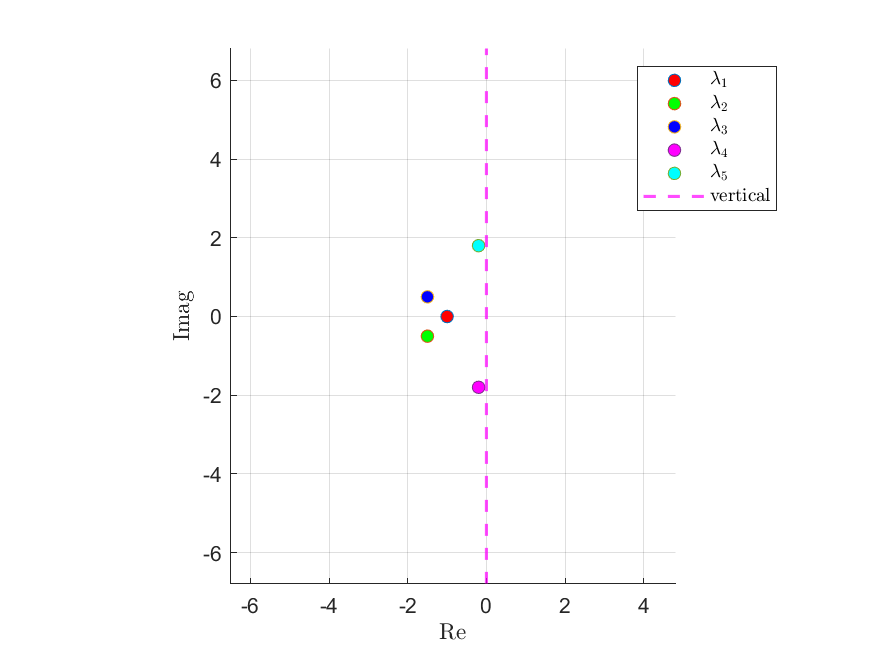
\includegraphics[width=0.9\linewidth]{roots_open2.png} 
    \caption{Разомкнутая система}
  \end{subfigure}
  \begin{subfigure}{0.5\textwidth}
    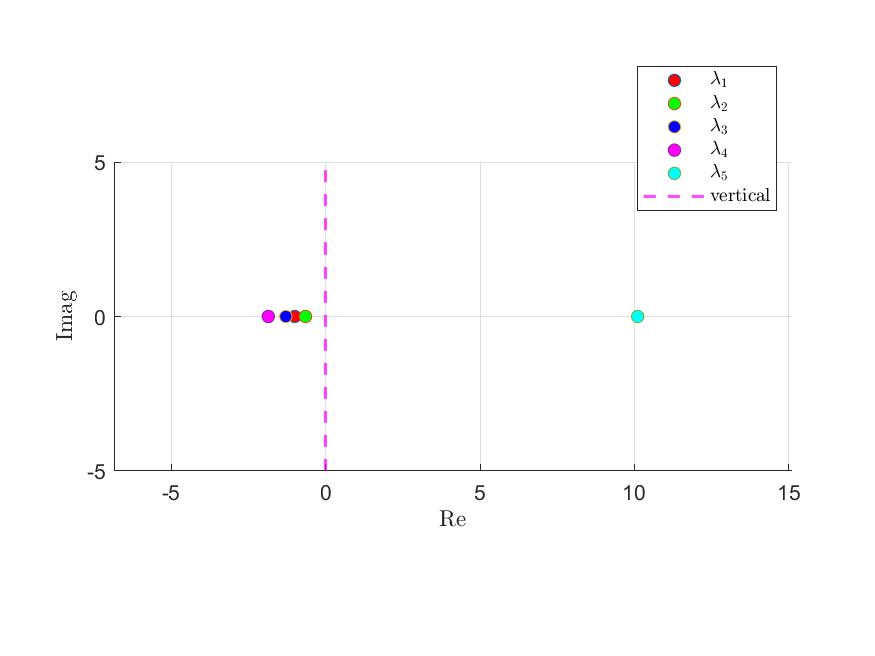
\includegraphics[width=0.9\linewidth]{roots_closed2.png}
    \caption{Замкнутая система}
  \end{subfigure}
  \caption{Карты полюсов для системы}
\end{figure}

\newpage
\subsection{Годограф Найквиста}
\begin{figure}[ht]
    \centering
    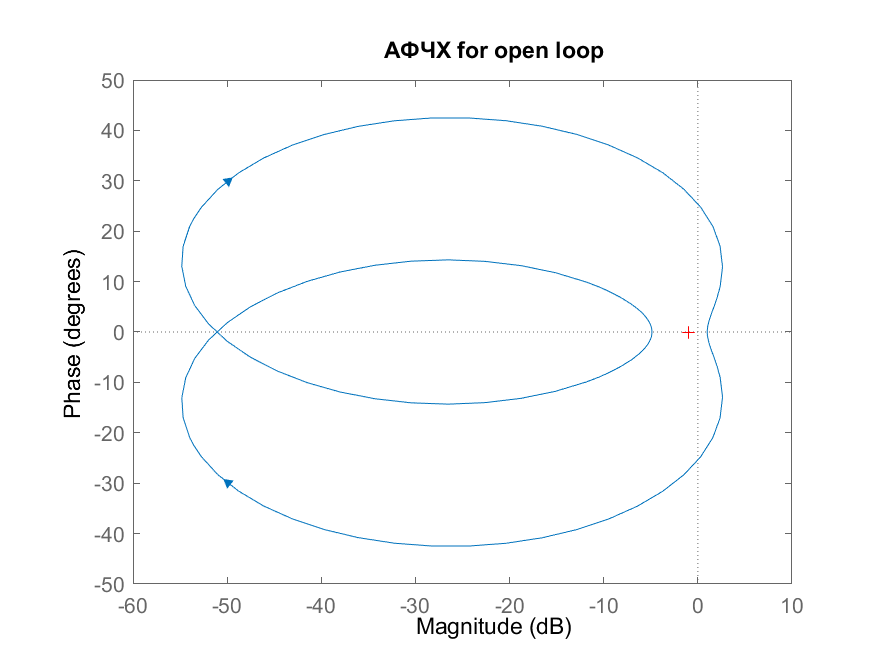
\includegraphics[width=1.0\textwidth]{nyquist_open2.png}
    \caption{Годограф Найквиста для системы}
  \end{figure}

Годограф Найквиста охватывает внутрь себя точку (-1, 0) и делает вокруг неё один оборот по часовой стрелке. 
По критерию Найквиста это значит, что у замкнутой системы количество неустойчивых полюсов станет на один больше, чем у разомкнутой(было 0, станет 0+1=1 неустойчивых полюсов). 

Именно такой результат мы в итоге и получили.

\newpage
\subsection{Переходные характеристики}

\begin{figure}[hbt!]
  \begin{subfigure}{.500\linewidth}
    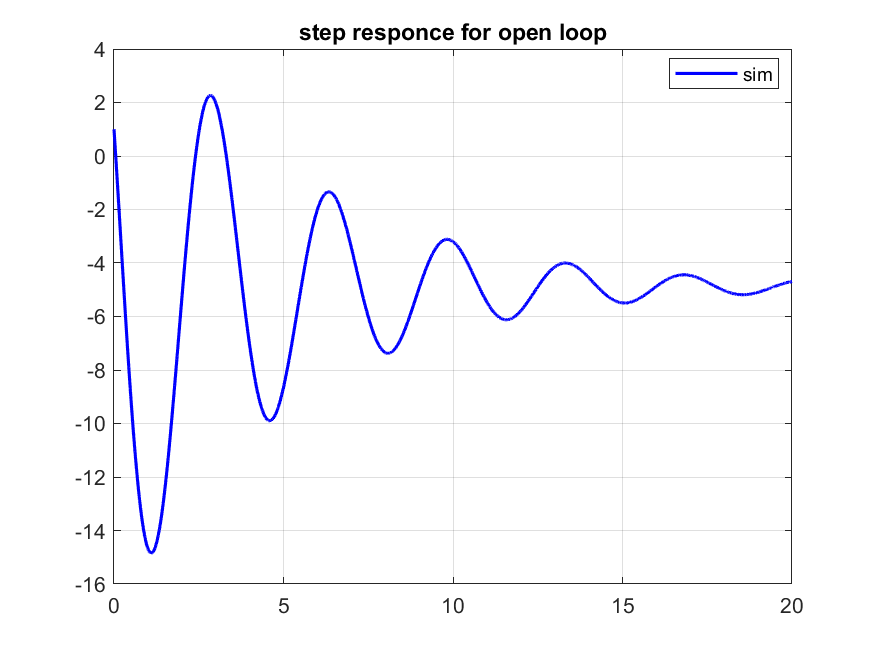
\includegraphics[width=\linewidth]{step_responce_open2.png}
    \caption{}
  \end{subfigure}\hfill % <-- "\hfill"
  \begin{subfigure}{.500\linewidth}
    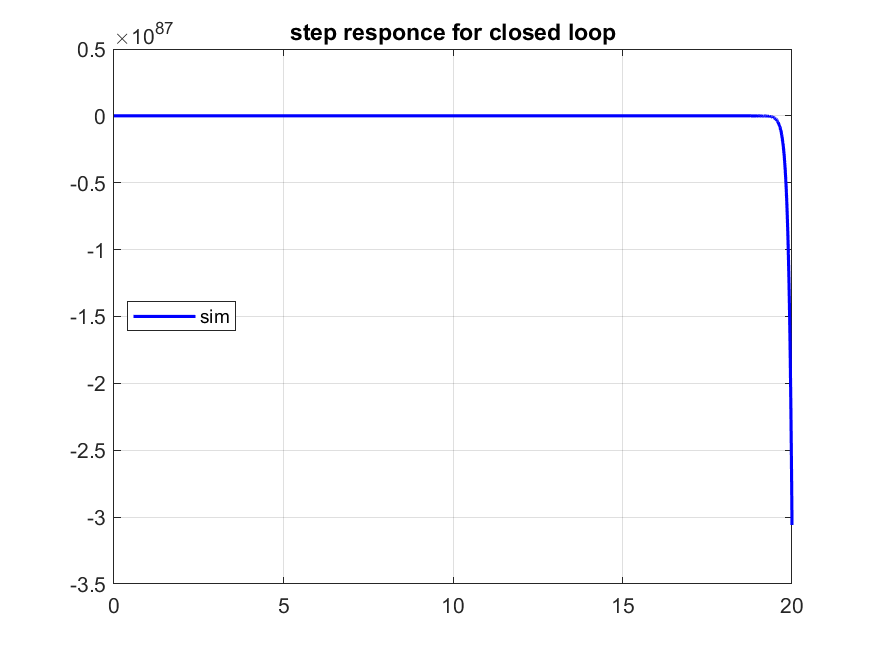
\includegraphics[width=\linewidth]{step_responce_closed2.png}
    \caption{}
  \end{subfigure}
  
  \medskip 
  \begin{subfigure}{.500\linewidth}
    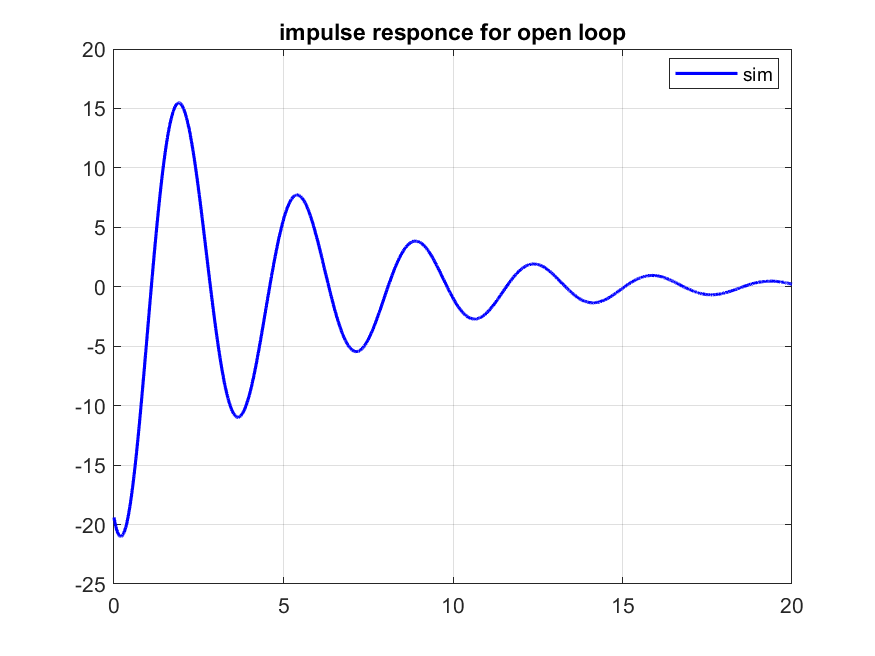
\includegraphics[width=\linewidth]{impulse_responce_open2.png}
    \caption{}
  \end{subfigure}\hfill 
  \begin{subfigure}{.500\linewidth}
    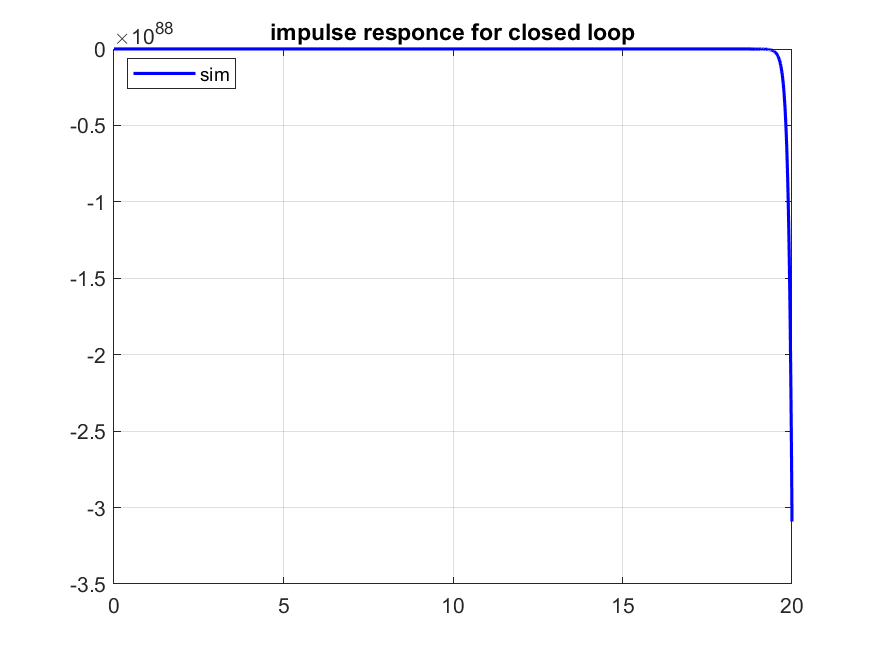
\includegraphics[width=\linewidth]{impulse_responce_closed2.png}
    \caption{}
  \end{subfigure}
  
  \caption{Сравнение - переходные характеристики}
  \end{figure}
По переходным функциям можем сделать вывод, что разомкнутая система была устойчивой, но замкнутая уже потеряла устойчивость из-за годографа...


\newpage
\subsection{Логарифмический критерий Найквиста}
Построим ЛАФЧХ для аналитики:
\begin{figure}[ht]
    \centering
    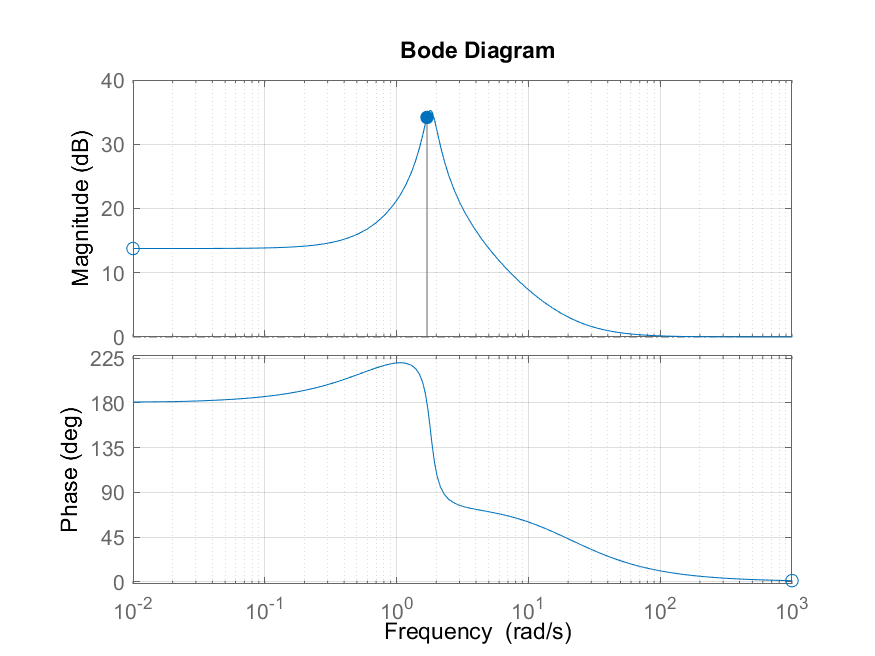
\includegraphics[width=1.0\textwidth]{log_nyquist2.png}
    \caption{ЛАФЧХ для системы}
  \end{figure}

Из графика делаем вывод, что система является неустойчивой по логарифмическому критерию Найквиста, 
мы стартуем из значения $180^\circ$, что является критическим отрезком, значит мы считаем переход за $+\frac{1}{2}$, 
далее на отметке ЛФЧХ в $180^\circ$ у нас будет отрицательный переход $-1$, но для устойчивости нам нужно, чтобы разность между переходами была равна $\frac{r}{2}= \frac{0}{2} = 0$, у нас будет $\frac{1}{2} -1 = -0.5$, этого недостаточно.


\section{Система третья}
Данная система должна иметь 4 неустойчивых полюсов у разомкнутой системы и 0 у замкнутой. 
Значит годограф Найквиста должен сделать 4 оборота против часовой стрелке вокруг $(-1, 0)$.
\subsection{Передаточная функция}
$$
W_{open}(s) = \frac{s^5 +35s^4 +159s^3 +277s^2 +212s+60}{s^5 -\frac{12}{5}s^4+\frac{179}{50}s^3-\frac{193}{50}s^2-\frac{66}{25}s+\frac{41}{5}}
$$
$$
W_{closed}(s) = \frac{s^5 +35s^4 +159s^3 +277s^2 +212s+60}{2s^5 +\frac{163}{5}s^4+\frac{8129}{50}s^3+\frac{13657}{50}s^2+\frac{5234}{25}s+\frac{341}{5}}
$$
\subsection{Карты полюсов}
\begin{figure}[h]
  \begin{subfigure}{0.5\textwidth}
    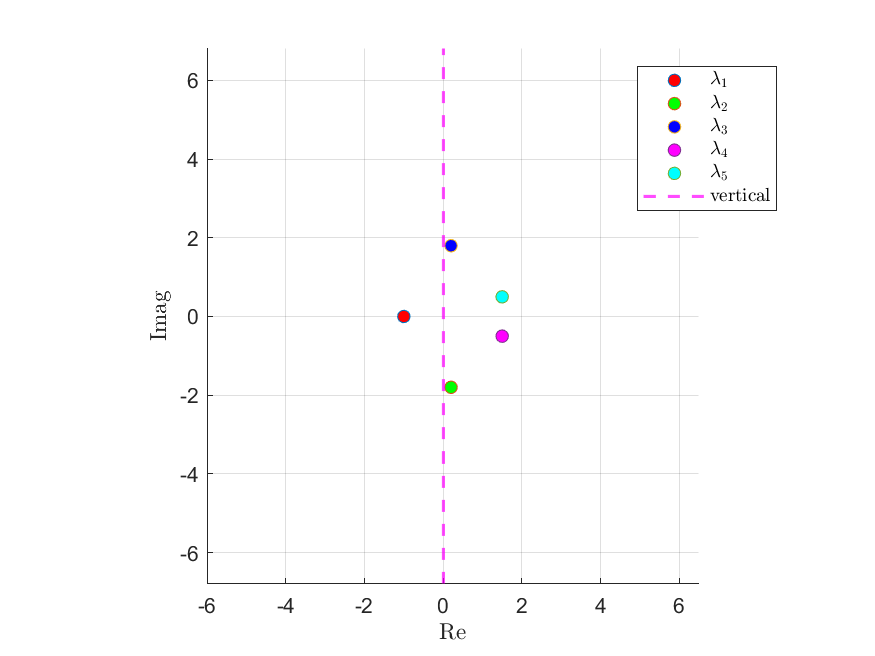
\includegraphics[width=0.9\linewidth]{roots_open3.png} 
    \caption{Разомкнутая система}
  \end{subfigure}
  \begin{subfigure}{0.5\textwidth}
    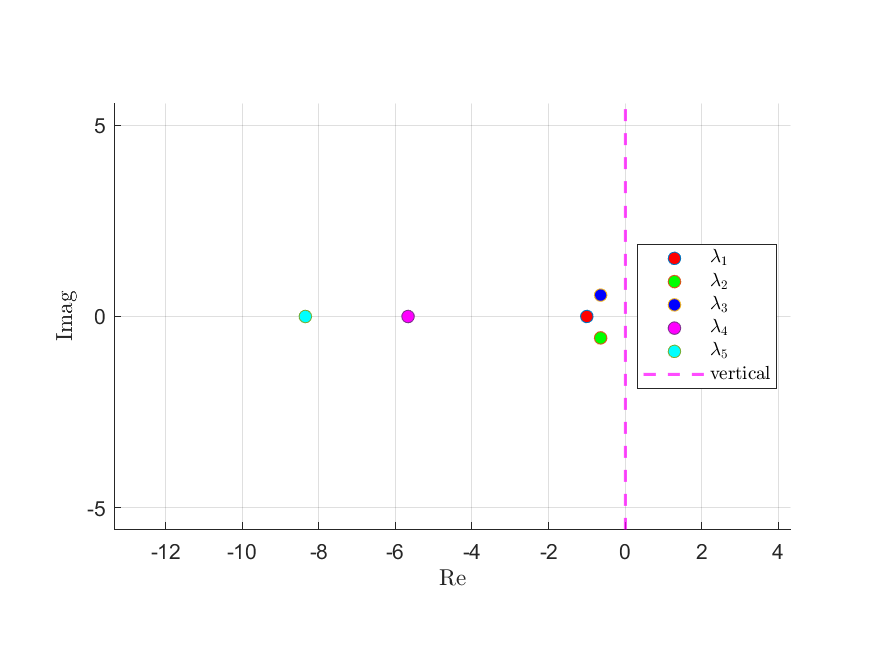
\includegraphics[width=0.9\linewidth]{roots_closed3.png}
    \caption{Замкнутая система}
  \end{subfigure}
  \caption{Карты полюсов для системы}
\end{figure}

\newpage
\subsection{Годограф Найквиста}
\begin{figure}[ht]
    \centering
    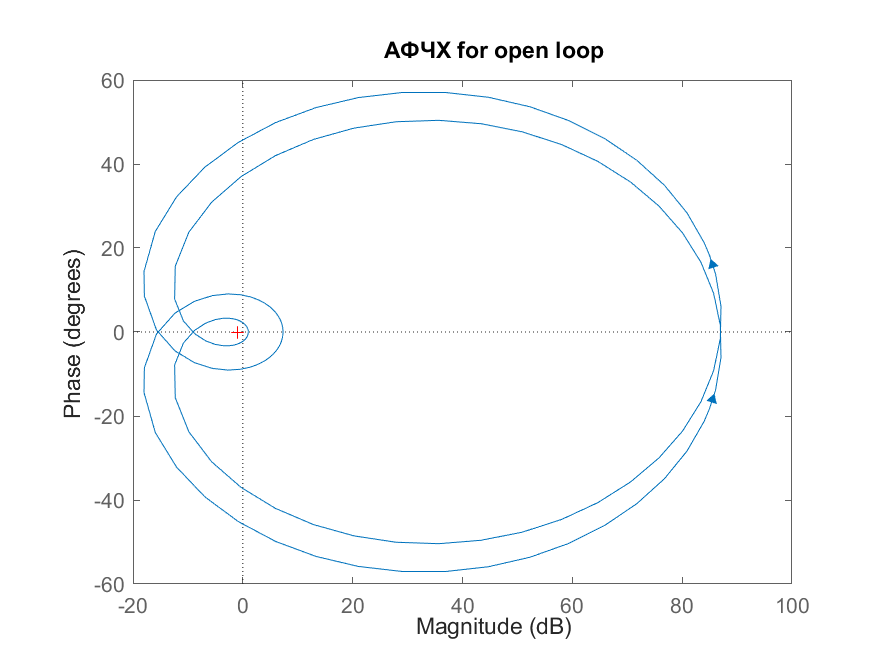
\includegraphics[width=1.0\textwidth]{nyquist_open3.png}
    \caption{Годограф Найквиста для системы}
\end{figure}

Годограф Найквиста охватывает внутри себя точку (-1, 0) и делает вокруг неё 4 оборота против часовой стрелки. 
По критерию Найквиста это значит, что у замкнутой системы количество неустойчивых полюсов станет на четыре меньше, чем у разомкнутой(было 4, станет 4-4=0 неустойчивых полюсов). 

Именно такой результат мы в итоге и получили.

\newpage
\subsection{Переходные характеристики}

\begin{figure}[hbt!]
  \begin{subfigure}{.500\linewidth}
    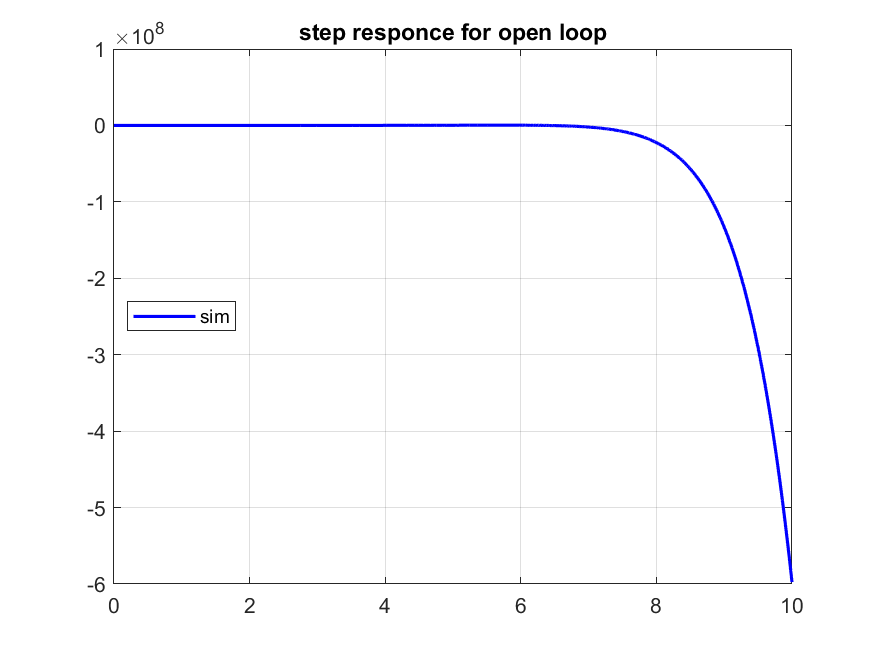
\includegraphics[width=\linewidth]{step_responce_open3.png}
    \caption{}
  \end{subfigure}\hfill % <-- "\hfill"
  \begin{subfigure}{.500\linewidth}
    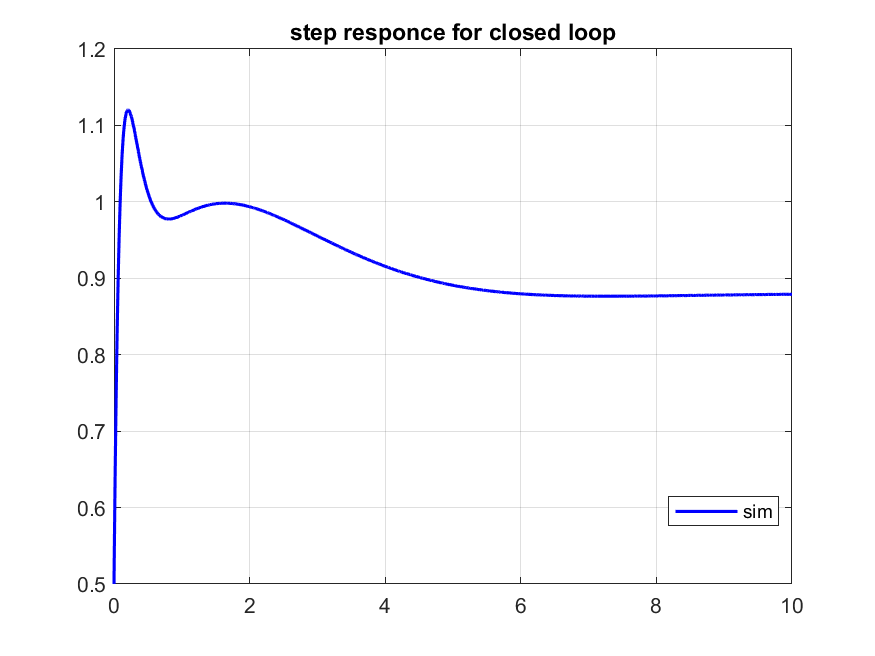
\includegraphics[width=\linewidth]{step_responce_closed3.png}
    \caption{}
  \end{subfigure}
  
  \medskip 
  \begin{subfigure}{.500\linewidth}
    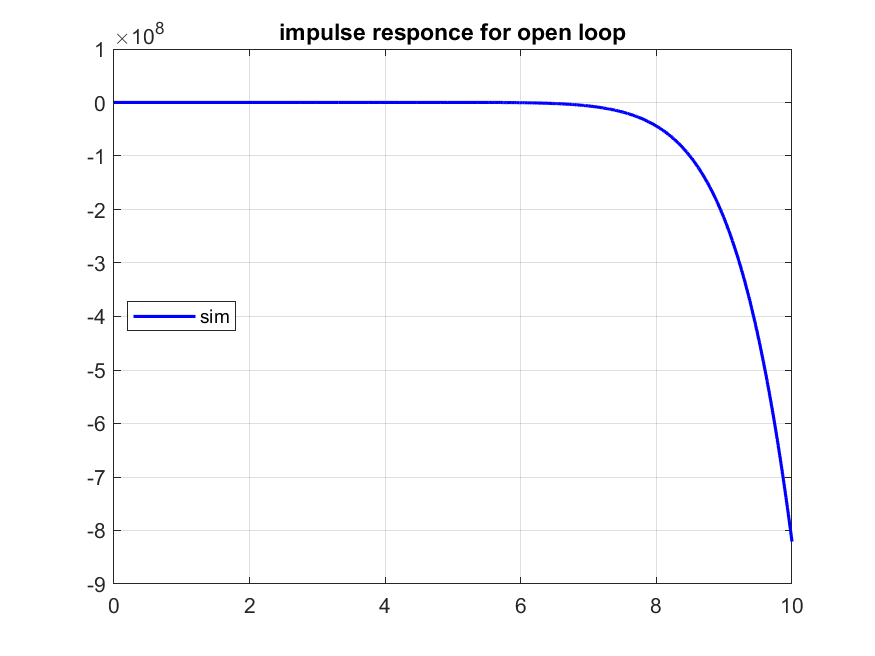
\includegraphics[width=\linewidth]{impulse_responce_open3.png}
    \caption{}
  \end{subfigure}\hfill 
  \begin{subfigure}{.500\linewidth}
    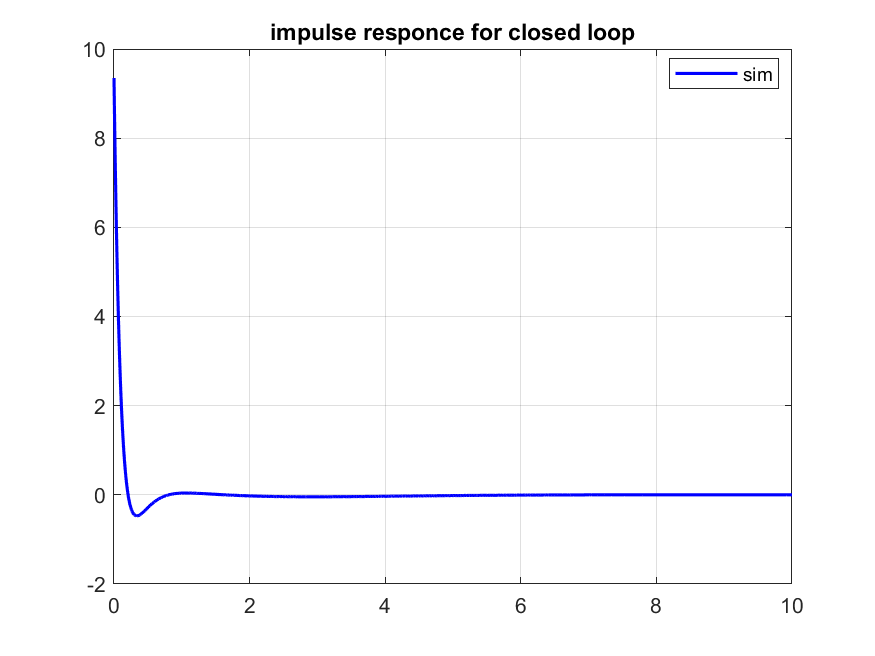
\includegraphics[width=\linewidth]{impulse_responce_closed3.png}
    \caption{}
  \end{subfigure}
  \caption{Сравнение - переходные характеристики}
  \end{figure}
По переходным функциям можем сделать вывод, что разомкнутая система была неустойчивой, но замкнутая уже приобрела устойчивость из-за годографа.


\newpage
\subsection{Логарифмический критерий Найквиста}
Построим ЛАФЧХ для аналитики:
\begin{figure}[ht]
    \centering
    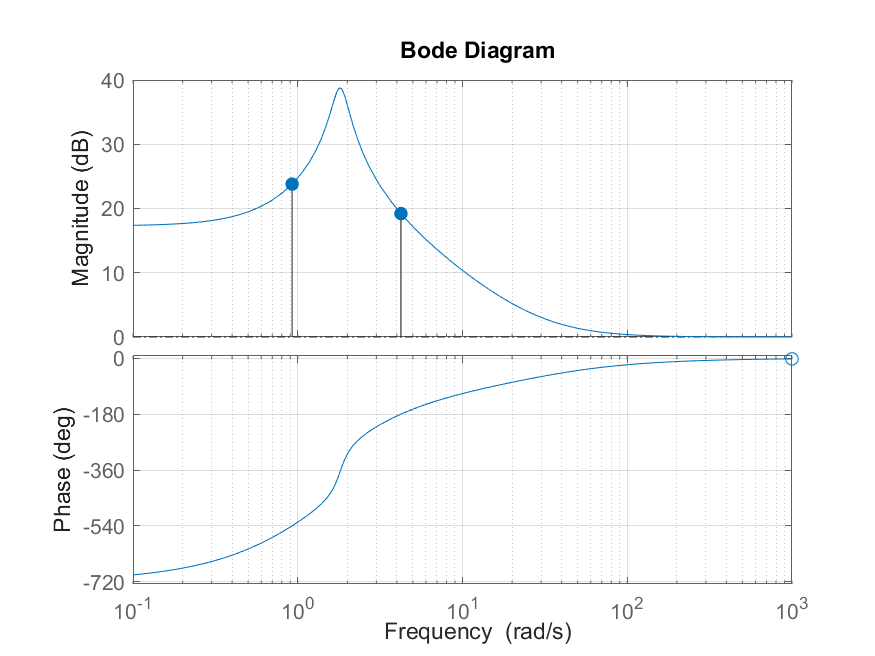
\includegraphics[width=1.0\textwidth]{log_nyquist3.png}
    \caption{ЛАФЧХ для системы}
  \end{figure}

Из графика делаем вывод, что система является устойчивой по логарифмическому критерию Найквиста, 
мы стартуем из значения $-720^\circ$, далее на отметке ЛФЧХ в $-540^\circ$ и $-180^\circ$ у нас будет два положительных перехода $+2$, но для устойчивости нам нужно, чтобы разность между переходами была равна $\frac{r}{2}= \frac{4}{2} = 2$, у нас будет $2-0 = 2$, этого вполне достаточно.

\endinput